%----------------------------------------------------------------------------
%----------------------------------------------------------------------------
%----------------------------------------------------------------------------
%----------------------------------------------------------------------------
%bb defines the bounding box for the pdf
%viewport defines the area of the pdf used
%in sidewaysfigure the last entry in bb moves the caption toward/away the pic
%in sidewaysfigure the second entry in bb moves the pic toward/away the caption
%----------------------------------------------------------------------------
\begin{figure}
\scalebox{1}[1]{
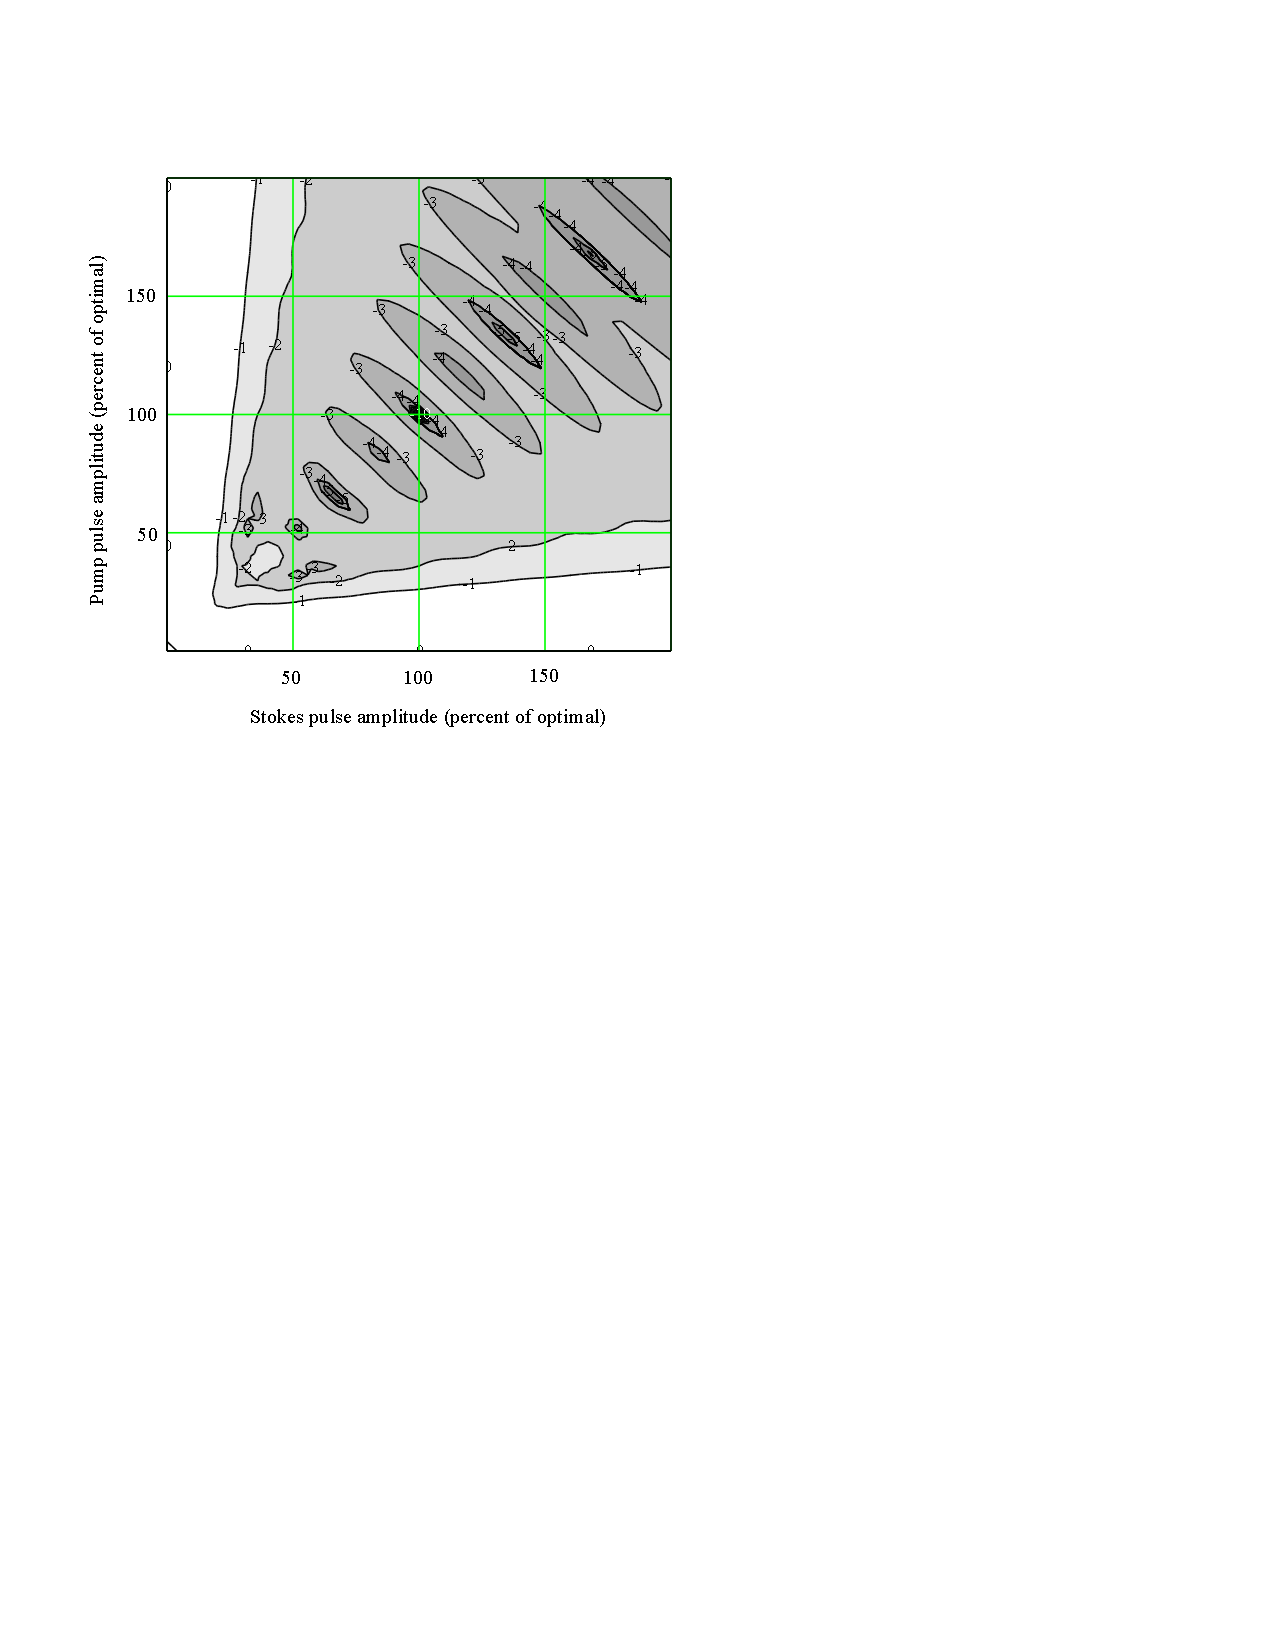
\includegraphics[bb=-15 450 489 700]
{amp_surface/amp_surface.pdf}
}
\caption[Residue surface for various pulse intensities]{Residue surface for various pulse intensities.}
\label{amp_surface}
\end{figure}
%----------------------------------------------------------------------------

%----------------------------------------------------------------------------
One important feature of the STIRAP process is the independence of the inversion on pulse height (first discussed in Chapter \ref{computer chapter}). Figure \ref{amp_surface} shows the surface
\begin{equation}
\Phi^{\prime}
=
1 - P_2(t_N)
\label{phi prime}
\end{equation}
with respect to the amplitudes of the two pulses in the two color solution (STIRAP) shown in Figure \ref{solution 2 pulses}. $\Phi^{\prime}$ is defined in a manner similar to Equation \ref{residue cost} - in fact, the surface in Figure \ref{amp_surface} is similar to, but not the same as, the surface in Figure \ref{amp amp}. Since $\Phi^{\prime}\sim0$ means the inversion was mostly complete, we see that for a majority of the transitions shown in Figure \ref{amp_surface} the inversion was complete to better than 1 part per thousand. Figure \ref{scale_two-color} shows $\Phi^{\prime}$ for the case of simultaneous scaling of the pulses. Compare this to Figure \ref{scale_three-color} where the three color STIRAP is analyzed in a similar way, and we see that the three color STIRAP does not exhibit the same ``robustness'' to pulse amplitude scaling.
%----------------------------------------------------------------------------
%----------------------------------------------------------------------------
%bb defines the bounding box for the pdf
%viewport defines the area of the pdf used
%in sidewaysfigure the last entry in bb moves the caption toward/away the pic
%in sidewaysfigure the second entry in bb moves the pic toward/away the caption
%----------------------------------------------------------------------------
\begin{figure}
\scalebox{0.8}[0.8]{
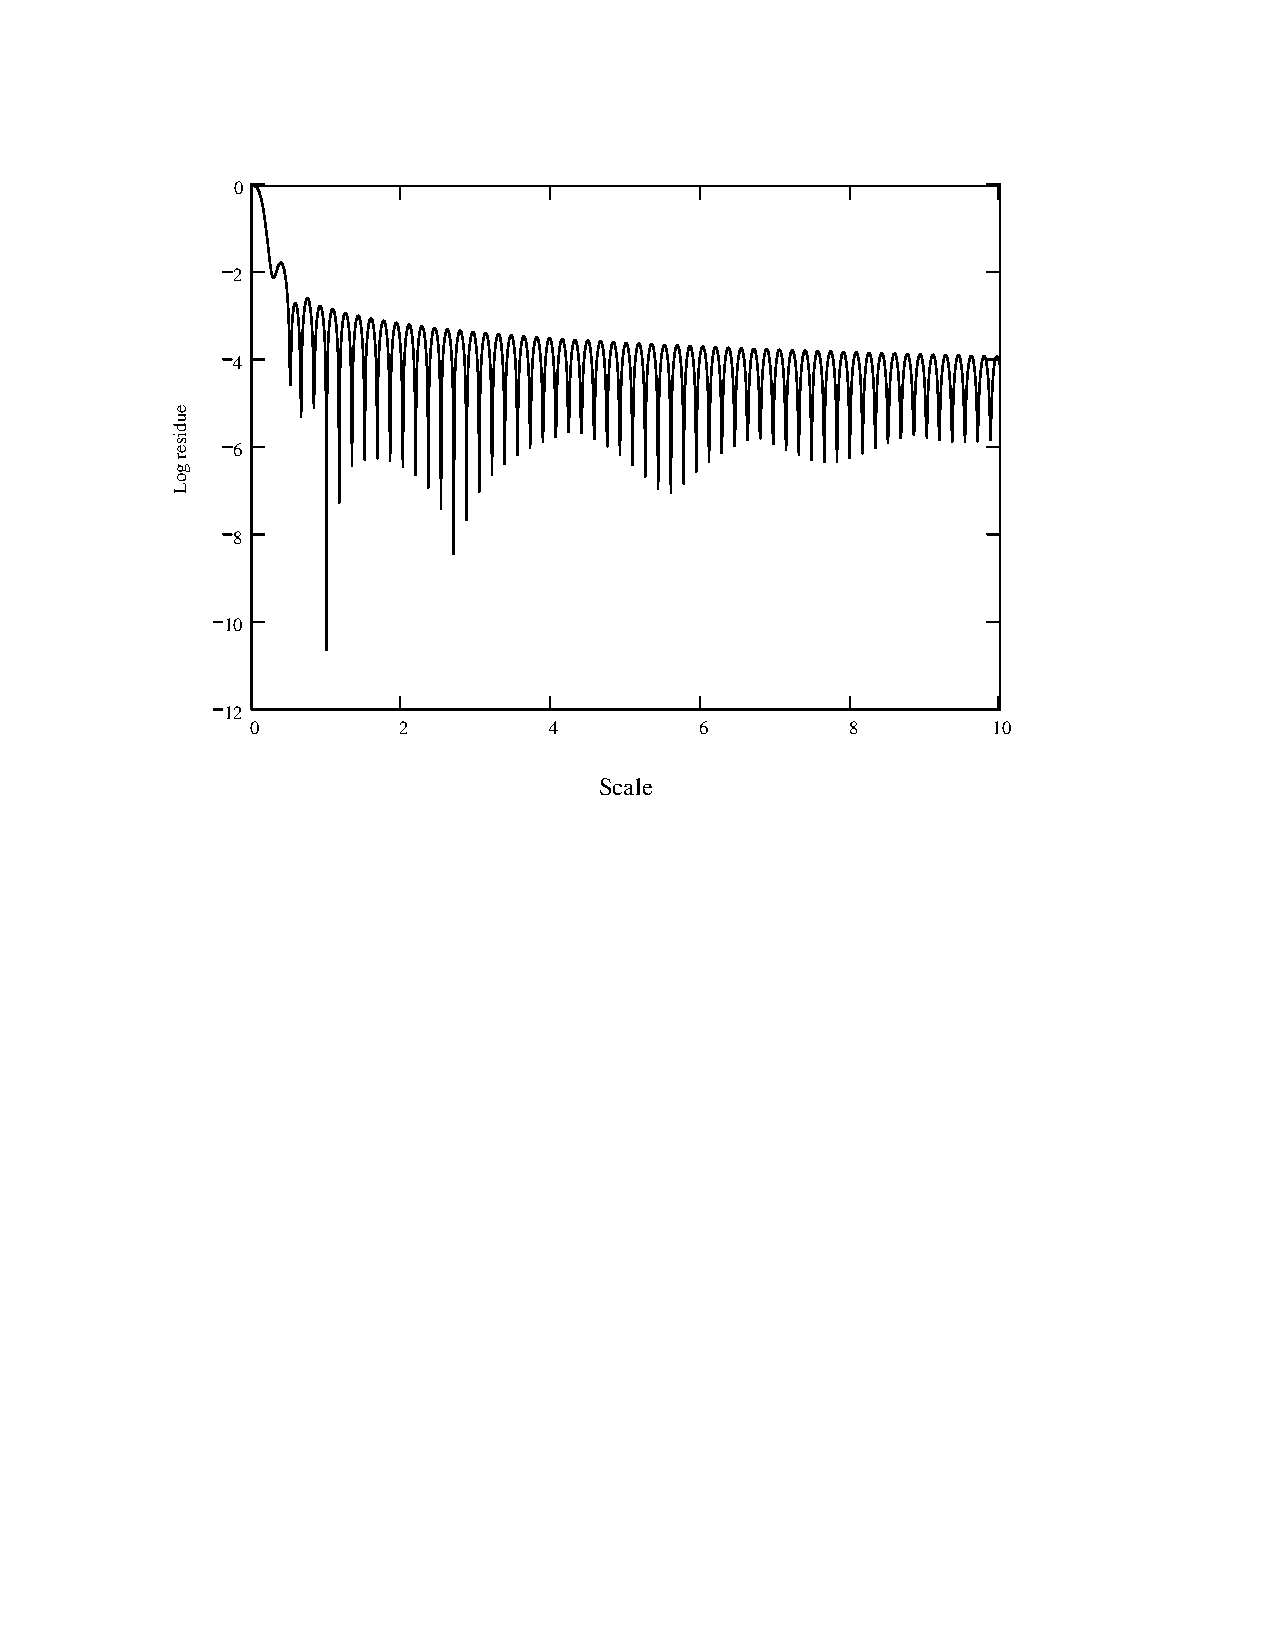
\includegraphics[bb=30 415 489 715]
{scale_two-color/scale_two-color.pdf}
}
\caption[Amplitude ``robustness'' of the two color STIRAP]{Amplitude ``robustness'' of the two color STIRAP. The optimal solution in Figure \ref{solution 2 pulses} is allowed to vary in pulse height by the ``scale'' factor (both pulses are scaled simultaneously) and the resulting residue, as defined by Equation \ref{phi prime} is plotted as a function of the scale. The narrow downward ``spikes'' are real; however, their depth may not be acurately displayed here due to ``aliasing'' effects between the regular spacing of computer generated points and the sharp spikes. In short, the residue is around $10^{-3}$ for most of the range of the ``scale'' factor, except for numerous ``pits'' where the residue drops to $10^{-6}$ or less.}
\label{scale_two-color}
\end{figure}
%----------------------------------------------------------------------------

%----------------------------------------------------------------------------
%----------------------------------------------------------------------------
%----------------------------------------------------------------------------
%bb defines the bounding box for the pdf
%viewport defines the area of the pdf used
%in sidewaysfigure the last entry in bb moves the caption toward/away the pic
%in sidewaysfigure the second entry in bb moves the pic toward/away the caption
%----------------------------------------------------------------------------
\begin{figure}
\scalebox{0.8}[0.8]{
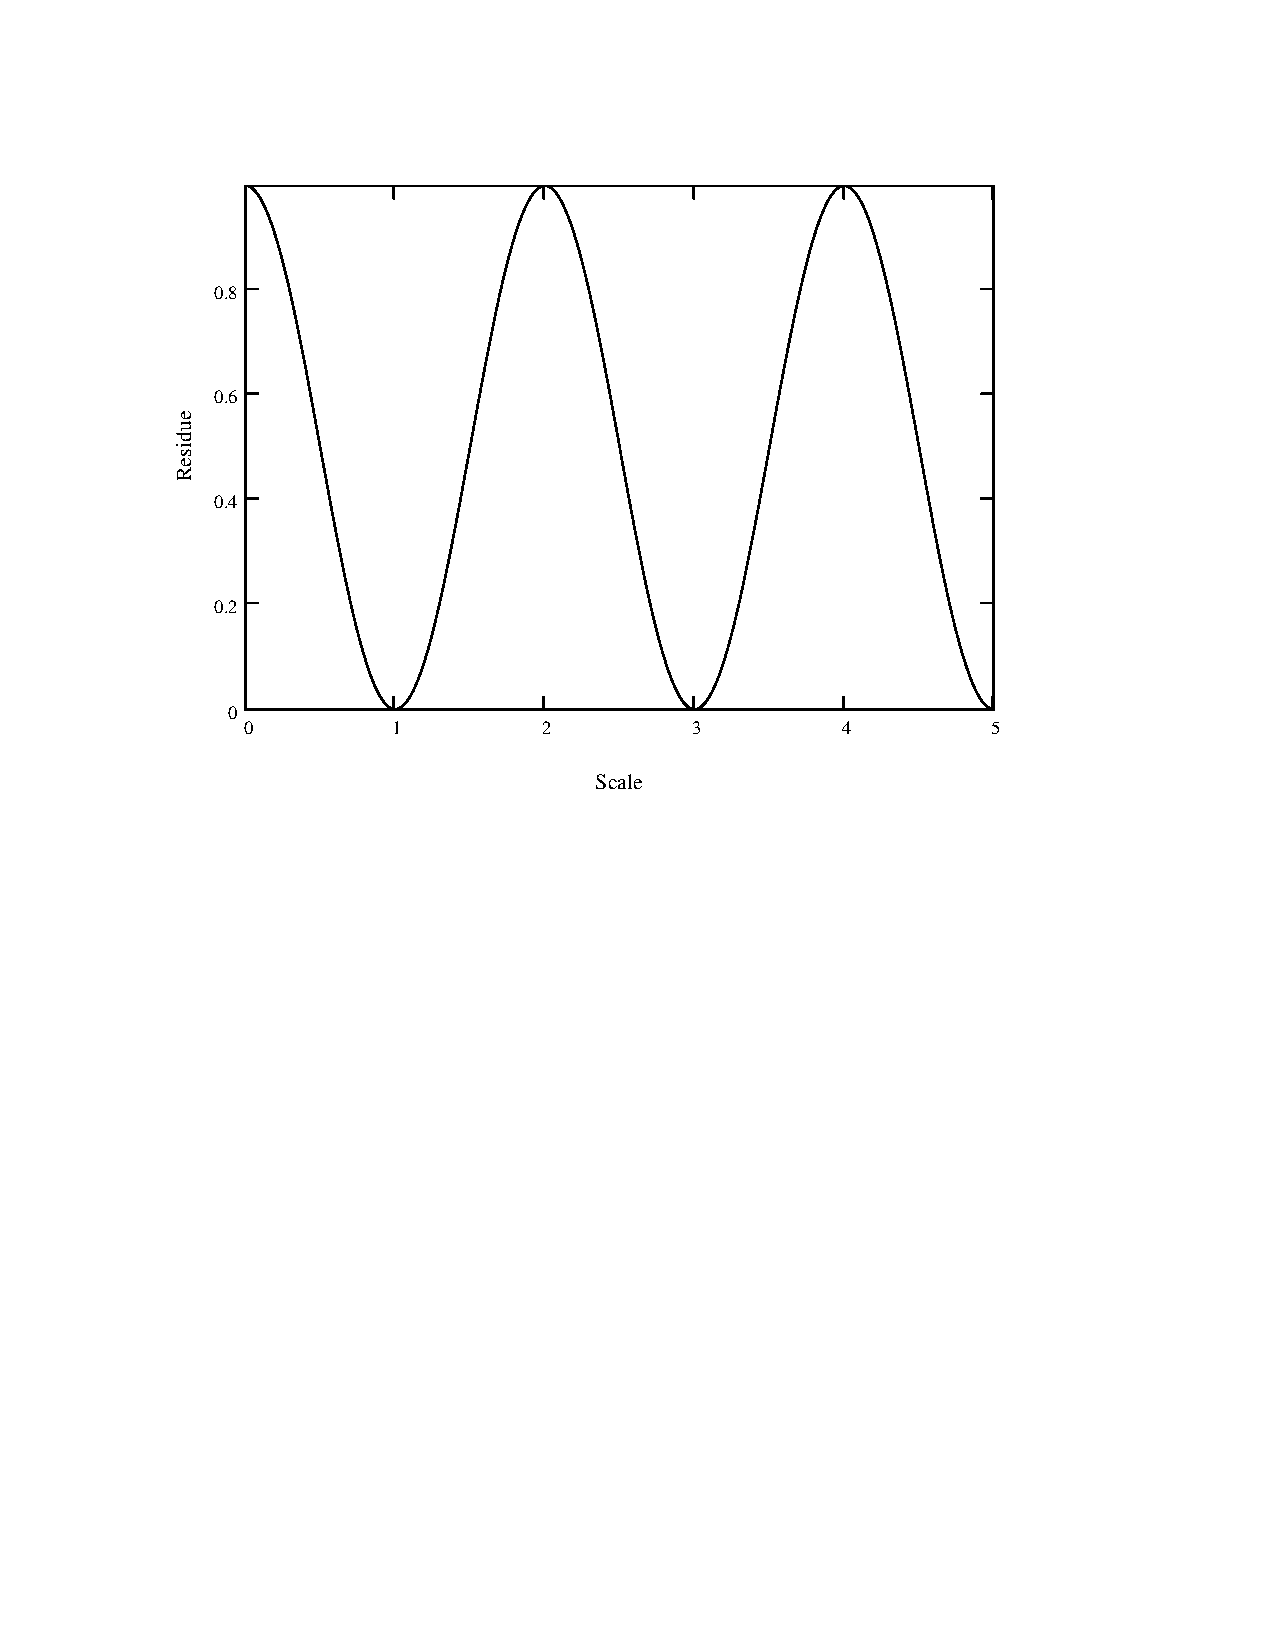
\includegraphics[bb=30 415 489 715]
{scale_three-color/scale_three-color.pdf}
}
\caption[Amplitude ``non-robustness'' of the three color STIRAP]{Amplitude ``non-robustness'' of the three color STIRAP. The optimal solution in Figure \ref{solution three pulses} is allowed to vary in pulse height by the ``scale'' factor (all three pulses are scaled simultaneously) and the resulting residue, as defined by Equation \ref{phi prime} is plotted as a function of the scale.}
\label{scale_three-color}
\end{figure}
%----------------------------------------------------------------------------

%----------------------------------------------------------------------------

%----------------------------------------------------------------------------
%----------------------------------------------------------------------------
